\title{\pkg{eurostat}: Eurostat Open Data R Tools}
\author{Leo Lahti, Janne Huovari, Markus Kainu, Przemyslaw Biecek}

\maketitle

%An abstract of less than 150 words.
\abstract{Governmental institutions have started to release increasing amount of
their data resources for the public as open data in the recent
years. This is opening novel opportunities for research and citizen
science. The eurostat R package provides a suite of tools to access open data from Eurostat, including functions to search, download, and manipulate these data sets in an automated and reproducible manner. The online documentation provides further examples on how to visualize, summarize and interpret these spatio-temporal data sets. The package builds on and extends the preceding SmarterPoland and statfi packages and has been extensively tested by the user community. This package contributes to the growing ecosystem of R packages that provide generic tools for reproducible computational research in social science and humanities.}


Efficient tools to access and analyse data collections available in
the public domain can greatly benefit reproducible
research \citep{Gandrud13}. When the data is available, the complete
analytical workflow spanning from raw data to the final publication
can be made available. Standardization and automatization of common
data analysis tasks via dedicated software packages can help to
automate the analysis workflow, thus greatly facilitate
reproducibility and code sharing and making data analysis more
transparent and efficient. 

Here, we introduce the eurostat R package that implements R tools to
access open data from
Eurostat \footnote{\url{http://ec.europa.eu/eurostat}}. Eurostat
provides a rich collection of demographic and economic data through
its open data portal. The portal currently includes ... data sets on
... between years ...

Despite many efforts to this direction, a dedicated R package for
eurostat open data has been missing. Our work extends our earlier CRAN
packages statfi \citep{statfi} and smarterpoland
\citep{smarterpoland}. Compared to this earlier work, we have now
implemented an expanded set of tools specifically focusing on the
eurostat data collection. The eurostat R package hence brings together
earlier, independent efforts by the package developers. It has been
actively developed by several contributors and based on the community
feedback in Github, with its first CRAN release in 2014. We are now
reporting the first mature version of the package that has been
improved and tested by multiple users, and includes features like
cache, handling dates, and using the tidy data
principles \citep{wickham2014}, with the help of the tidyr R
package \citep{tidyr}.

The datamart \citep{datamart} and the quandl
\citep{quandl} R packages provide generic tools that can be used to access
certain versions of eurostat data. In contrast to these generic
database packages, our the eurostat package provides functionality
that is particularly tailored for this data collection. There is also
a development version for R package
\pkg{reurostat}\footnote{https://github.com/Tungurahua/reurostat} but this
does not seem to be actively maintained. The package
depends on or imports the following external R packages:
\CRANpkg{devtools} \citep{devtools}, \CRANpkg{dplyr} \citep{dplyr},
\CRANpkg{knitr} \citep{knitr}, \CRANpkg{ggplot2} \citep{ggplot2},
\CRANpkg{mapproj} \citep{mapproj}, \CRANpkg{plotrix} \citep{plotrix},
\CRANpkg{reshape2} \citep{reshape2}, \CRANpkg{rmarkdown}
\citep{rmarkdown}, \CRANpkg{stringi} \citep{stringi},
\CRANpkg{testthat} \citep{testthat}, and \CRANpkg{tidyr}
\citep{tidyr}. The eurostat R package is
part of the rOpenGov project
\citep{Lahti13icml}, which provides reproducible research tools for
computational social science and digital humanities.


The package provides tools to search and retrieve data from the
Eurostat open data portal, to convert identifiers in human-readable
formats and to select, modify and visualize the data. In this
manuscript, we provide a brief overview of the core functionality in
the current CRAN release version (1.2.1). For further examples, see
the package
vignette\footnote{https://github.com/rOpenGov/eurostat/vignette/eurostat\_tutorial.Rmd}.

To install the CRAN release version, type in R:

\code{
install.packages("eurostat")
}


\section{Search and download commands}

The complete table of contents of the database can be downloaded in R
with the function \code{get\_eurostat\_toc()} [HERE LINK TO EUROSTAT
PAGE WHERE THE DATA CAN BE BROWSED ONLINE]. The
function \code{search\_eurostat()} can be used to make a more focused
search over the table of contents. To retrieve data sets for
'disposable income', for instance, use:

\begin{example}
library(eurostat)
income <- search_eurostat("disposable income", type = "dataset")
\end{example}


The queried data type is specified in the above example with
the \code{type} argument. The options for this argument
include \dfn{'table'}, \dfn{'dataset'} or \dfn{'folder'}, referring to
different levels of hierarchy in the data organization: a table
resides in dataset, and the datasets are stored in a
folder. The \code{type} argument limits the search on a selected data
set type. Values from the code column list identifiers for specific
data sets. These can be used in subsequent download
commands. Alternatively, the dataset identifier codes can also be
browsed at the Eurostat
website\footnote{http://ec.europa.eu/eurostat/data/database}; check
the codes in the Data Navigation Tree listed after each dataset (in
parentheses).

To retrieve the data set with a particular identifier (tsdtr210, for
instance), use

\code{
dat <- get\_eurostat(id = 'tsdtr210', time\_format = "num")
}

Since the original data is annual in this example, we have selected a
numeric time variable as this is more convient for annual time series
than the default date format. The function call returns a table on
passenger transport statistics in various countries. The first lines
of the output are shown in Table~\ref{tab:getdatatable}.

\begin{table}[ht]
\centering
\begin{tabular}{rlllrr}
\toprule
  \hline
 & unit & vehicle & geo & time & values \\ 
  \hline
  1 & PC & BUS\_TOT & AT & 1990.00 & 11.00 \\ 
  2 & PC & BUS\_TOT & BE & 1990.00 & 10.60 \\ 
  3 & PC & BUS\_TOT & BG & 1990.00 &  \\ 
  4 & PC & BUS\_TOT & CH & 1990.00 & 3.70 \\ 
  5 & PC & BUS\_TOT & CY & 1990.00 &  \\ 
  6 & PC & BUS\_TOT & CZ & 1990.00 &  \\ 
   \hline
\bottomrule   
\end{tabular}
\caption{Example on \code{get_eurostat} function output with \code{dat <- get\_eurostat(id = 'tsdtr210', time\_format = "num")}} 
\label{tab:getdatatable}
\end{table}

To improve the interpretability of the output, the eurostat variable
identifiers could be further replaced with human-readable labels based
on definitions from Eurostat dictionaries with
the \code{label\_eurostat()} function. The data is provided in the
standard data.frame format, so that all standard tools for data
subsetting and reshaping are supported.



\section{Visualization}

To make a triangle map from the \CRANpkg{plotrix} \citep{plotrix}
package provides an example on visualizing passenger transport data
distributions (Figure~\ref{fig:plotrix}):

\begin{figure}
\setkeys{Gin}{width=0.5\textwidth}
\begin{center}
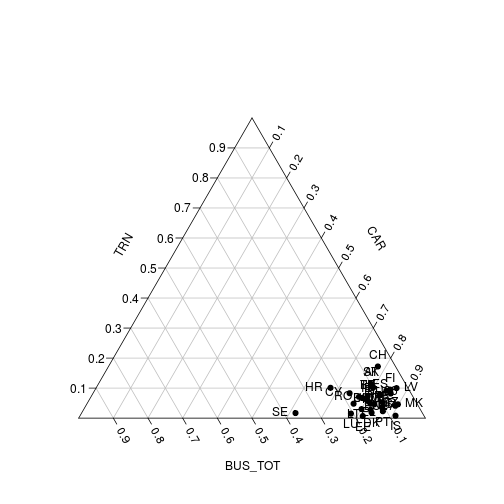
\includegraphics{2015-manu-search2-1}
\end{center}
\caption{Test caption2.}
\label{fig:plotrix}
\end{figure}

The package or its predecessors have already been applied in several case studies by us and independent developers. Financial Times, for instance, used R to access data from Eurostat\footnote{http://blog.revolutionanalytics.com/2015/04/financial-times-tracks-unemployment-with-r.html} using functions from SmarterPoland, the direct predecessor of our revised and expanded eurostat package.

The archivist R package\footnote{http://pbiecek.github.io/archivist} for archivisation of objects has exemplified\footnote{http://pbiecek.github.io/archivist/justGetIT.html} its functionality by using eurostat to plot the number of people killed by road accidents, showing a decreasing trend of road accidents in many countries (Figure~\ref{fig:roadaccidents}).

We can also look at the distribution of BMI between different age groups (Figure~\ref{fig:bmi}).


\begin{figure}
\setkeys{Gin}{width=0.5\textwidth}
\begin{center}
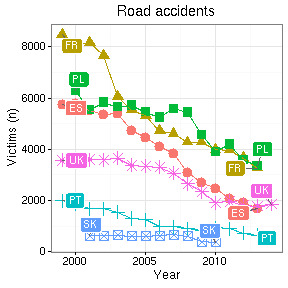
\includegraphics{2015-manu-roadacc-1}
\end{center}
\caption{Road accidents caption}
\label{fig:roadaccidents}
\end{figure}


\begin{figure}
\setkeys{Gin}{width=0.5\textwidth}
\begin{center}
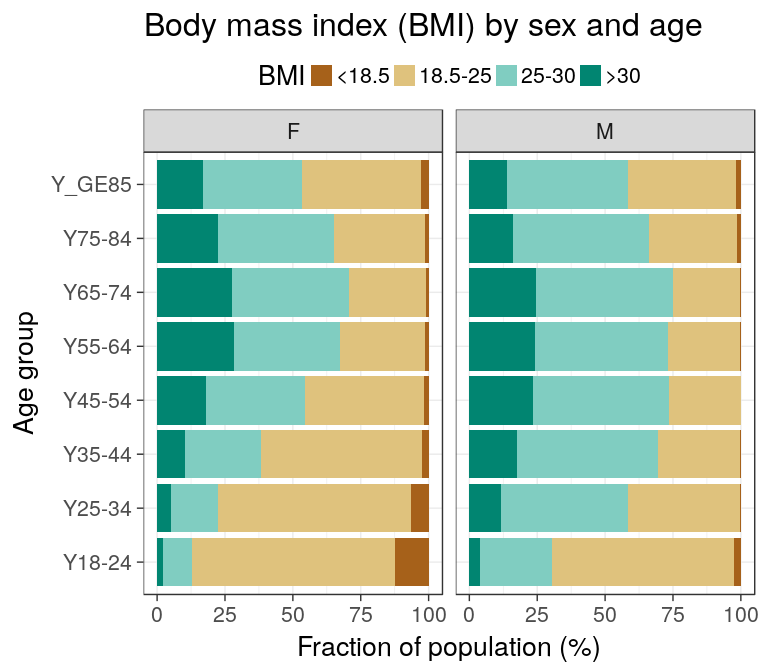
\includegraphics{2015-manu-bmi-1}
\end{center}
\caption{BMI caption}
\label{fig:bmi}
\end{figure}


Data sets containing geographic information can be visualized on a
map. Most indicators are of country-year -type, although some
indicators have data also at lower level of regional breakdown
%\footnote{http://ec.europa.eu/eurostat/ramon/nomenclatures/index.cfm\?TargetUrl=DSP\_GEN\_DESC\_VIEW\_NOHDR\&StrNom=NUTS\_33\&StrLanguageCode=EN}.

\begin{figure}
\setkeys{Gin}{width=0.5\textwidth}
\begin{center}
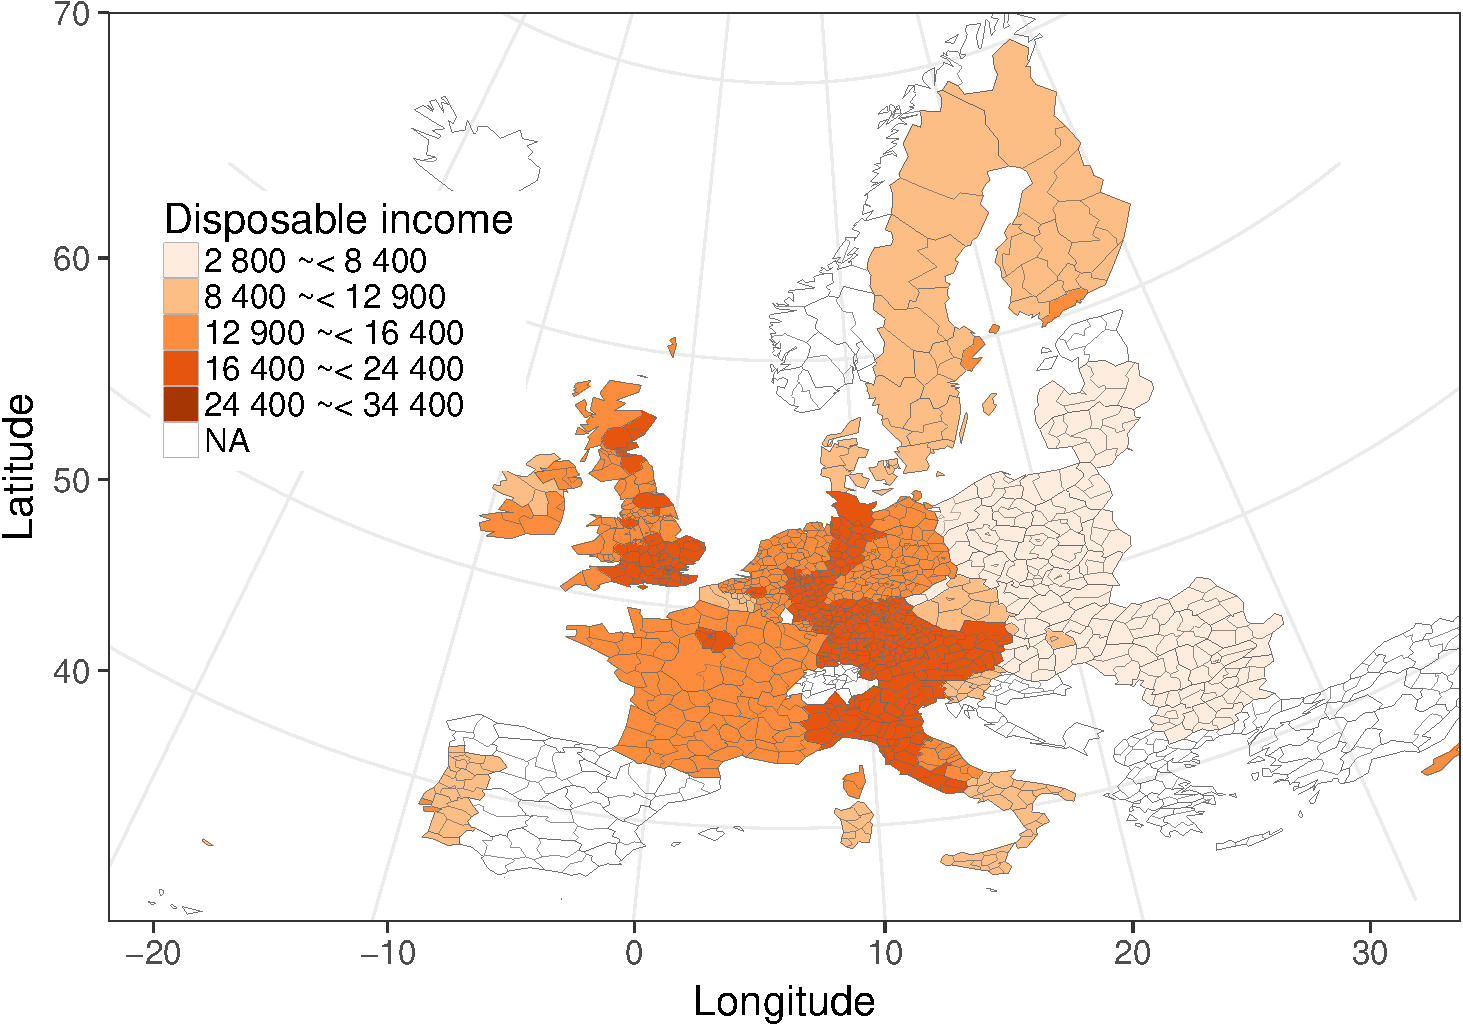
\includegraphics{2015-manu-mapexample-1}
\caption{Test caption for map example.}
\label{fig:mapexample}
\end{center}
\end{figure}


The disposable income of private households at
NUTS2\footnote{http://en.wikipedia.org/wiki/Nomenclature\_of\_Territorial\_Units\_for\_Statistics}
level can be visualized, for instance, as in
Figure~\ref{fig:mapexample}. For a more detailed treatment of this
example, see our related blog
post\footnote{http://ropengov.github.io/r/2015/05/01/eurostat-package-examples}.

Here, we have combined the data retrieved with the eurostat package
with additional map visualization tools and utilities including
\CRANpkg{grid} \citep{grid}, \CRANpkg{maptools} \citep{maptools}, \CRANpkg{rgdal} \citep{rgdal},
\CRANpkg{rgeos} \citep{rgeos}, \CRANpkg{scales} \citep{scales}, and
\CRANpkg{stringr} \citep{stringr}.

Example on spatio-temporal data visualization: let us look at the
indicator
tgs00026\footnote{http://ec.europa.eu/eurostat/en/web/products-datasets/-/TGS00026},
(Disposable income of private households by NUTS 2 regions) from
Eurostat. We are looking at the disposable household income. In
addition to downloading and manipulating data from EUROSTAT, we
demonstrate how to access and use shapefiles of Europe published by
EUROSTAT at Administrative units / Statistical
units\footnote{http://ec.europa.eu/eurostat/web/gisco/geodata/reference-data/administrative-units-statistical-units}.


\section{Other functionality}

To facilitate fast plotting of standard European geographic areas, the package provides ready-made lists of the country codes used in the eurostat database for EFTA (efta\_countries), Euro area (ea\_countries), EU (eu\_countries) and EU candidate countries (candidate\_countries). This helps to select specific groups of countries for closer investigation. For conversions with other standard country coding systems, see the \CRANpkg{countrycode} R package \citep{countrycode}. To retrieve the eurostat country code list for EFTA (Table~\ref{tab:efta}), use:

\begin{example}
data(efta_countries)
\end{example}


% latex table generated in R 3.2.2 by xtable 1.8-0 package
% Mon Nov 23 15:10:36 2015
\begin{table}[ht]
\centering
\begin{tabular}{rll}
\toprule
  \hline
 & code & name \\ 
  \hline
  1 & IS & Iceland \\ 
  2 & LI & Liechtenstein \\ 
  3 & NO & Norway \\ 
  4 & CH & Switzerland \\ 
   \hline
\bottomrule   
\end{tabular}
\label{tab:efta}
\caption{EFTA countries.}
\end{table}


The downloaded data sets are stored in cache by default. This can help
to avoid repeated downloading of identical data and helps to speed up
the analysis. Another advantage is that by storing an exact copy of
the data on the hard disk, it is possible to reproduce the analysis
results afterwards even if the source database has been updated.



\section{Summary}

The eurostat R package provides convenient tools to access open data
from Eurostat. When automated access to the data sets is integrated
with data analytical tools from other packages, this allows a seamless
automation of the data analytical process from raw data access to
statistical analysis and the final publication.

The package source code can be freely used, modified and distributed
under the BSD-2-clause (modified FreeBSD) license. A reproducible
version of this article is available at .. and can be used to generate
the manuscript text along with up-to-date figures and tables with the
latest version of the eurostat data. Manuscript automation provides
transparent documentation with full algorithmic details on how to
access, preprocess, analyse, and report data and analyses, thus
serving a template for good reproducible research practice. The reproducible source code for this manuscript is available at eurostat github page\footnote{https://github.com/rOpenGov/eurostat/blob/master/vignettes/manuscript.Rmd}.

The package exemplifies also the challenges and possible solutions to
reproducible research and automated open data retrieval. Possible
future extensions and improvements include design of specific data
representation class structures. This could facilitate harmonization
of the data representation with similar governmental data sets and
subsequent tool development. The latest development version of the
package can be installed from Github by following the instructions at
the github site\footnote{https://github.com/rOpenGov/eurostat}. We welcome
issues, bug reports and other feedback via the development
site\footnote{https://github.com/ropengov/eurostat}.


\section*{Acknowledgements}

We are grateful to Eurostat\footnote{http://ec.europa.eu/eurostat} for
maintaining the open data portal and the
rOpenGov\footnote{https://github.ropengov.io} for supporting 
package development. This work has been partially funded by Academy of
Finland (decision 293316). We also wish to thank Juuso Parkkinen and Joona Lehtomaki for their feedback on this work.


\bibliography{lahti-huovari-kainu-biecek}

\address{Leo Lahti\\
  Department of Mathematics and Statistics\\
  PO Box 20014 University of Turku\\
  Finland\\}
\email{leo.lahti@iki.fi}

\address{Janne Huovari\\
  Affiliation\\
  Address\\
  Country\\}
\email{author2@work}

\address{Markus Kainu\\
  Affiliation\\
  Address\\
  Country\\}
\email{author3@work}

\address{Przemyslaw Biecek\\
  Faculty of Mathematics, Informatics, and Mechanics\\
  University of Warsaw\\
  Banacha 2, 02-097 Warsaw\\
  Poland\\}
\email{P.Biecek@mimuw.edu.pl}

